\documentclass[%
 reprint,
%superscriptaddress,
%groupedaddress,
%unsortedaddress,
%runinaddress,
%frontmatterverbose, 
%preprint,
%showpacs,preprintnumbers,
%nofootinbib,
%nobibnotes,
%bibnotes,
 amsmath,amssymb,
 aps,
%pra,
%prb,
%rmp,
%prstab,
%prstper,
%floatfix,
]{revtex4-1}

\usepackage{graphicx}% Include figure files
\usepackage{dcolumn}% Align table columns on decimal point
\usepackage{bm}% bold math
%\usepackage{hyperref}% add hypertext capabilities
%\usepackage[mathlines]{lineno}% Enable numbering of text and display math
%\linenumbers\relax % Commence numbering lines

%\usepackage[showframe,%Uncomment any one of the following lines to test 
%%scale=0.7, marginratio={1:1, 2:3}, ignoreall,% default settings
%%text={7in,10in},centering,
%%margin=1.5in,
%%total={6.5in,8.75in}, top=1.2in, left=0.9in, includefoot,
%%height=10in,a5paper,hmargin={3cm,0.8in},
%]{geometry}

\usepackage{cmap} % Поиск в PDF
\usepackage[T2A]{fontenc} % Кодировка
\usepackage[utf8]{inputenc} % Кодировка исходного текста
\usepackage[english, russian]{babel} % Локализация и переносы
\frenchspacing % Более тонкая настройка пробелов 
\usepackage{multirow}
\usepackage[warn]{mathtext}
\usepackage{amssymb}
\usepackage{ dsfont }
\usepackage{ textcomp }
\usepackage{ mathrsfs }

% Переопределение англоязычного начертания каппа, фи и эпсилон, 
% а также знаков сравнения
\renewcommand{\epsilon}{\ensuremath{\varepsilon}}
\renewcommand{\phi}{\ensuremath{\varphi}} 
\renewcommand{\kappa}{\ensuremath{\varkappa}}
\renewcommand{\le}{\ensuremath{\leslant}}
\renewcommand{\leq}{\ensuremath{\leqslant}}
\renewcommand{\ge}{\ensuremath{\geslant}}
\renewcommand{\geq}{\ensuremath{\geqslant}}
\renewcommand{\emptyset}{\ensuremath{\varnothing}}

\usepackage{textcomp} 
\usepackage{indentfirst} % Красная строка
\usepackage{amsmath} % Текст в формулах
\usepackage{graphicx} % Графика
\DeclareGraphicsExtensions{.pdf,.png,.jpg}
\usepackage{pgfplots}
\pgfplotsset{compat=1.13}

%\usepackage{times}

\begin{document}

\title{Изучение спектров атома водорода и молекулы йода}
\thanks{2.2, 2.3}

\author{Иван Едигарьев}
\affiliation{
 Московский Физико-Технический Институт\\
 Факультет Общей и Прикладной Физики, 526т\\
}
%\date{\today}

\begin{abstract}
В работе исследуются: а) сериальные закономерности в оптическом спектре водорода; б) спектр поглощения паров йода в видимой области.

\end{abstract}

\pacs{Valid PACS appear here}

\maketitle

\begin{enumerate}

\item 
\textbf{Градуировка спектрометра}\\
Проградуируем спектрометр по спектру неона и ртути и построим градуировочную кривую.

\item
\textbf{Спектр водорода}\\
Измерим положение линий $H_{\alpha}$, $H_{\beta}$, $H_{\gamma}$ и $H_{\delta}$. Определим длины волн этих линий с помощью калибровочного графика.
\begin{gather*}
\lambda_{\alpha} = 6568~\text{\AA},\\
\lambda_{\beta} = 4872~\text{\AA},\\
\lambda_{\gamma} = 4346~\text{\AA},\\
\lambda_{\delta} = 4113~\text{\AA}.
\end{gather*}

Убедимся в том, что отношения длин волн водородных линий соответствуют формуле сериальной закономерности.
\begin{gather*}
n_{\alpha} = 2.99,\\
n_{\beta} = 3.98,\\
n_{\gamma} = 4.98,\\
n_{\delta} = 5.92.
\end{gather*}

Для каждой из наблюдаемых линий водорода вычислим значение постоянной Ридберга, определим её среднее значение по всем измерениям и оценим погрешность измерения. Сравните результаты опыта с расчётным значением $R$.
\begin{gather*}
R_{\alpha} = 109622~\text{cm}^{-1},\\
R_{\beta} = 109469~\text{cm}^{-1},\\
R_{\gamma} = 109569~\text{cm}^{-1},\\
R_{\beta} = 109409~\text{cm}^{-1}.\\
\\
R = (109517 \pm 55)~\text{cm}^{-1},\\
R_{\text{table}} = 109737.3~\text{cm}^{-1}
\end{gather*}

\item
\textbf{Спектр йода}\\
По градуировочной кривой монохроматора определим длины волн линий поглощения йода, соответствующие делениям барабана монохроматора $n_{1,0}$, $n_{1,5}$, $n_{\text{гр}}$.
\begin{gather*}
\lambda_{1,0} = 6369~\text{\AA},\\
\lambda_{1,5} = 5495~\text{\AA},\\
\lambda_{\text{гр}} = 5158~\text{\AA}.
\end{gather*}

Вычислим в электронвольтах энергию колебательного кванта возбуждённого состояния молекулы йода:
\begin{gather*}
h\nu_2 = (h\nu_{1,5} - h\nu_{1,0})/5 = 0.06~\text{эВ}.
\end{gather*}

Используя полученные результаты, а также данные о том, что энергия колебательного кванта основного состояния $h\nu_1 = 0,027~\text{эВ}$, а энергия возбуждения атома $E_A = 0,94~\text{эВ}$ вычислим:

а) энергию электронного перехода 
\begin{gather*}
h\nu_{\text{эл}} = (E_2 - E_1) = \frac{1}{2}(h\nu_1 - h\nu_2) = 1.65~\text{эВ},
\end{gather*}

б) энергию диссоциации молекулы в основном состоянии
\begin{gather*}
D_1 = h\nu_{\text{гр}} - E_A = 1.46~\text{эВ},
\end{gather*}

в) энергию диссоциации молекулы в возбуждённом состоянии \begin{gather*}
D_2 = h\nu_{\text{гр}} - h\nu_{\text{эл}} = 0.75~\text{эВ}.
\end{gather*}

\begin{figure}[h]
\center{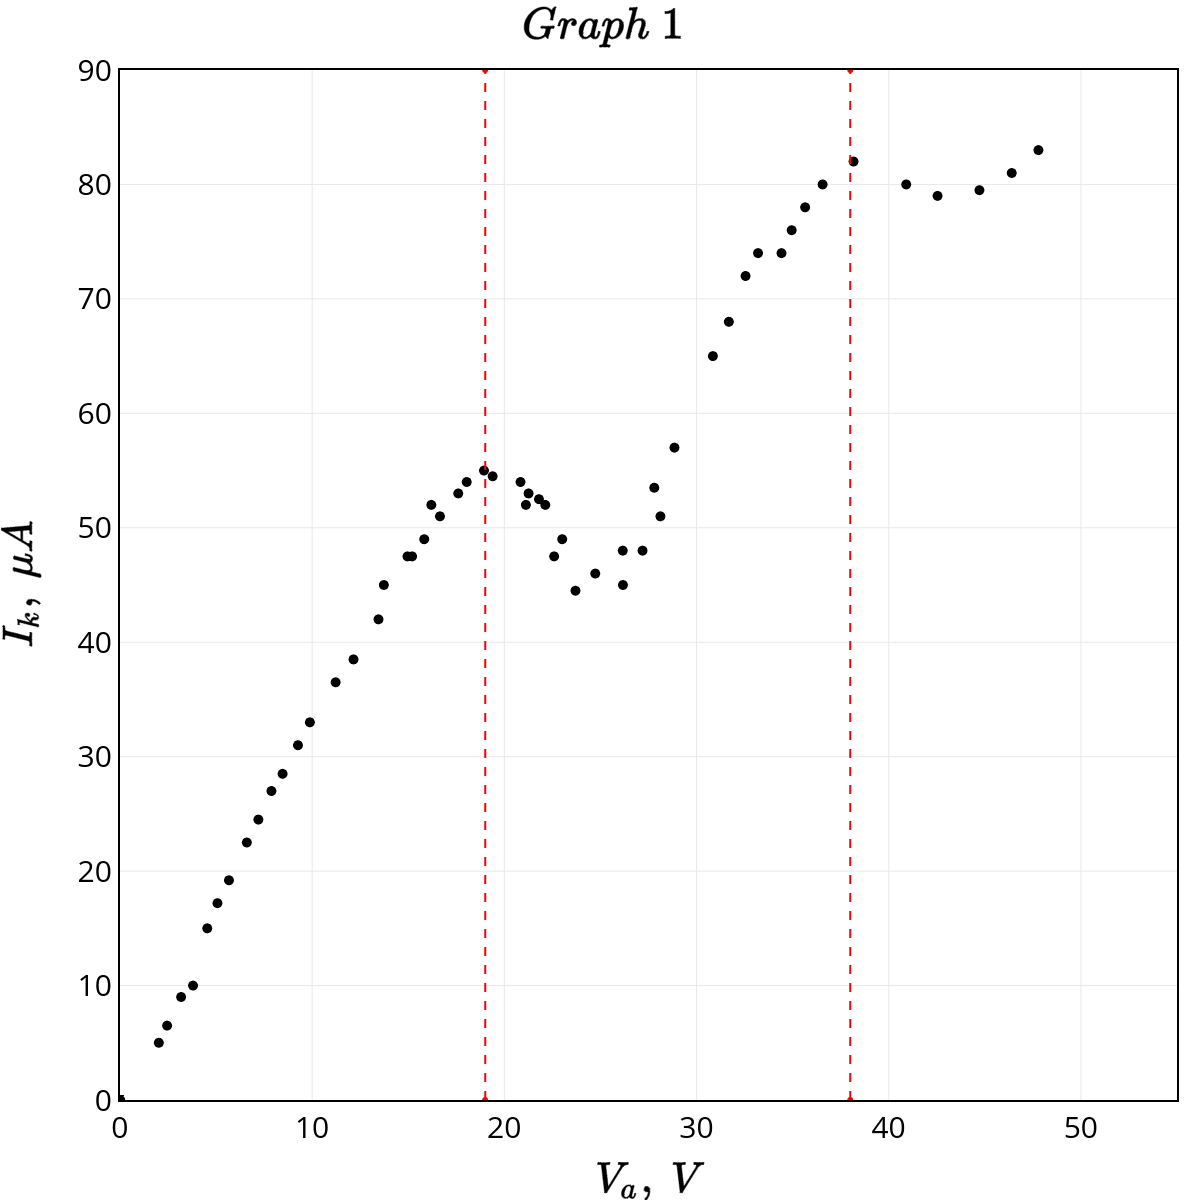
\includegraphics[scale=0.40]{my_plot1.png}}
\end{figure}

\end{enumerate}

\end{document}